% =============================================================================
% 3 Analyse des bestehenden Erwärmungsprüfstands
% =============================================================================
\section{Analyse des bestehenden Erwärmungsprüfstands}
\label{chap:analyse_pruefstand}

In diesem Kapitel wird der bestehende Erwärmungsprüfstand hinsichtlich seines
technischen Aufbaus, des betrieblichen Prüfablaufs und der Einstellung der
einzelnen Abgangsströme untersucht. Ziel der Analyse ist es, die Ursachen für
den wiederkehrenden manuellen Nachstellbedarf zu bestimmen und daraus
Anforderungen an die nachfolgende Konzeptentwicklung abzuleiten. Die
normativen Grundlagen des Erwärmungsnachweises sowie die allgemeinen
elektrischen und thermischen Zusammenhänge wurden bereits in
Kapitel~\ref{chap:technische_grundlagen} erläutert.

Die Betrachtung folgt zunächst dem Energiepfad vom betrieblichen
Drehstromnetz über die regelbare Hochstromeinspeisung bis zu den parallel
belasteten Abgangseinheiten des MCC-Feldes. Anschließend wird der derzeitige
Prüfablauf beschrieben. Darauf aufbauend werden der thermisch bedingte
Stromdrift, die Kopplung der parallelen Lastzweige und die Grenzen der
vorhandenen Gesamtstromregelung analysiert. Das Kapitel schließt mit
lösungsneutral formulierten Anforderungen, anhand derer die in
Kapitel~\ref{chap:entwicklung_stellkonzept} untersuchten Stellkonzepte
bewertet werden können.


% -----------------------------------------------------------------------------
% 3.1 Aufbau und Funktionsweise
% -----------------------------------------------------------------------------
\subsection{Aufbau und Funktionsweise}
\label{sec:aufbau_funktionsweise_pruefstand}

Der bestehende Prüfstand dient der Durchführung von Erwärmungsprüfungen an
Niederspannungs-Schaltgerätekombinationen. Die für den Prüfling benötigten
hohen Ströme werden bei einer niedrigen Spannung erzeugt. Dadurch lässt sich
die für die Erwärmung maßgebende Strombelastung bereitstellen, ohne den
Prüfstromkreis mit der betrieblichen Netzspannung beaufschlagen zu müssen.

Der funktionale Energiepfad ist in
Abbildung~\ref{fig:ist_energiepfad} dargestellt. Die Einspeisung erfolgt aus
dem betrieblichen \SI{400}{\volt}-Drehstromnetz. Ein motorisch verstellbarer
Säulenstelltransformator verändert die Spannung auf der Primärseite des
nachgeschalteten Festtransformators. Dieser transformiert die Spannung auf
das für die Hochstromprüfung benötigte niedrige Niveau. Unmittelbar hinter
dem Festtransformator werden die Ströme der drei Außenleiter erfasst. Über
ein Anbindefeld gelangt der Strom anschließend in die Prüfkombination aus
Leistungsschalterfeld und MCC-Feld. Im MCC-Feld teilt er sich auf die
parallel gespeisten Abgangseinheiten und einen über die Hauptsammelschiene
geführten Rückstrompfad mit Kurzschlussbrücke auf
\parencite[Bestandsaufnahme: Hochstromeinspeisung und
Prüfanordnung]{rj_pruefstand_2026}.

\begin{figure}[H]
    \centering
    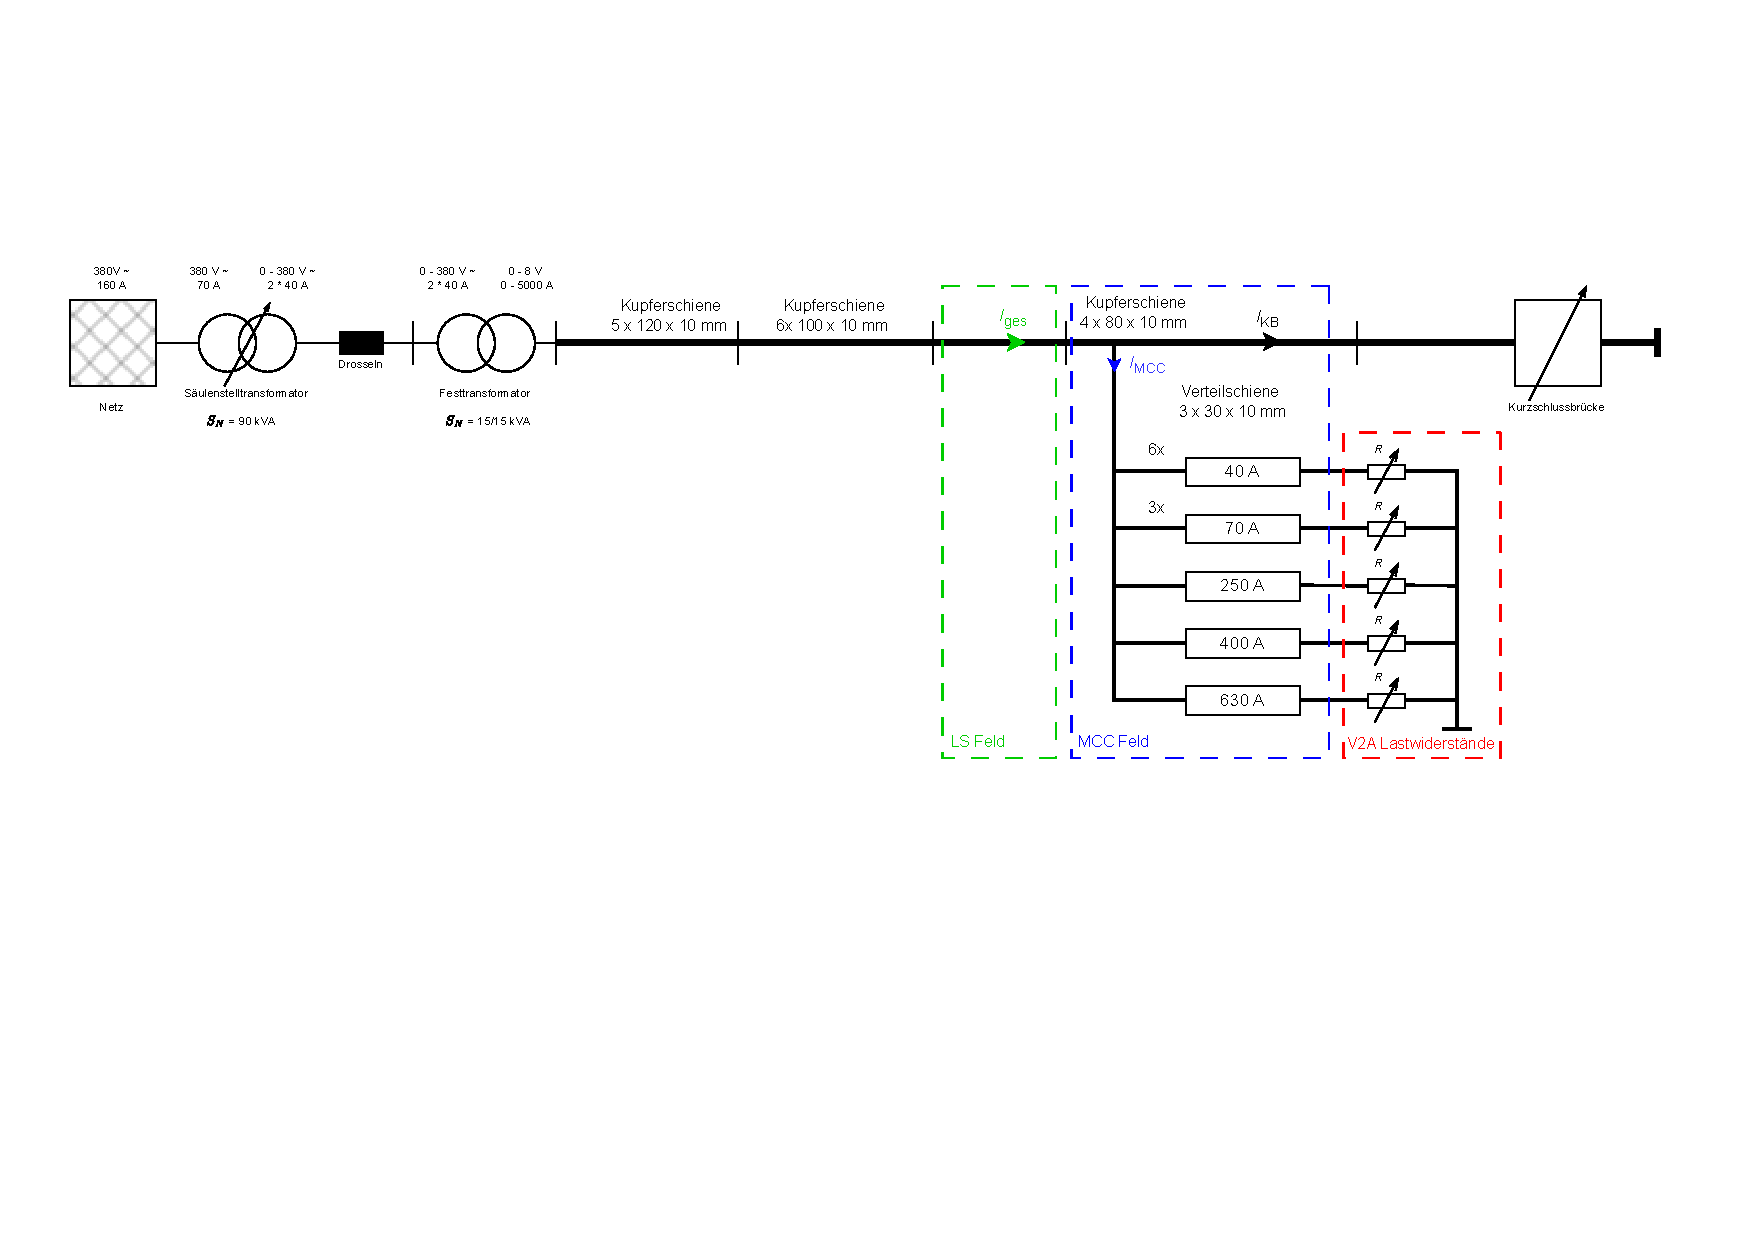
\includegraphics[width=\textwidth]
    {03_Ressourcen/drawio/ESB_Ist-Zustand.pdf}
    \caption{Funktionaler Energiepfad des bestehenden
    Erwärmungsprüfstands (eigene Darstellung auf Grundlage der
    betrieblichen Bestandsaufnahme)}
    \label{fig:ist_energiepfad}
\end{figure}

Der Säulenstelltransformator besitzt drei Wicklungssäulen, die den drei
Außenleitern zugeordnet sind. An jeder Wicklungssäule befinden sich zwei
Stromabnehmer, die gemeinsam durch einen motorischen Antrieb entlang der
freiliegenden Wicklung verfahren werden. Insgesamt sind somit sechs
Stromabnehmer und drei motorische Antriebe vorhanden. Die Stellung der
Stromabnehmer bestimmt die dem Festtransformator zugeführte Spannung. Da die
drei Antriebe mechanisch voneinander getrennt sind, können Unterschiede
zwischen den Außenleitern innerhalb der vorhandenen Stellgrenzen beeinflusst
werden. Aus dem mechanischen Aufbau allein lässt sich jedoch nicht ableiten,
dass im SPS-Programm drei vollständig unabhängige Regelkreise umgesetzt sind.

Die wesentlichen Typenschilddaten des Säulenstelltransformators sind in
Tabelle~\ref{tab:ist_saeulenstelltransformator} zusammengefasst. Die
primäre Nennspannung von \SI{380}{\volt} weicht von der heutigen
betrieblichen Netzspannung von \SI{400}{\volt} ab. Diese Abweichung ist bei
der Beurteilung des vorhandenen Betriebsmittels zu berücksichtigen; eine
weitergehende Bewertung seiner zulässigen Betriebsbeanspruchung ist nicht
Gegenstand dieser Arbeit.

\begin{table}[H]
    \centering
    \caption{Technische Daten des vorhandenen
    Säulenstelltransformators nach Typenschild}
    \label{tab:ist_saeulenstelltransformator}
    \begin{tabular}{p{0.48\textwidth}p{0.38\textwidth}}
        \toprule
        Kenngröße & Wert beziehungsweise Ausführung \\
        \midrule
        Hersteller und Typ & Ruhstrat TKDMT \\
        Baujahr & 1987 \\
        Nennleistung $S_\mathrm{N}$ & \SI{90}{\kilo\volt\ampere} \\
        Primäre Nennspannung $U_\mathrm{1N}$ & \SI{380}{\volt} \\
        Primärer Nennstrom $I_\mathrm{1N}$ & \SI{70}{\ampere} \\
        Sekundäre Ausgangsspannung &
        je Außenleiter zwei Ausgänge mit \SIrange{0}{380}{\volt} \\
        Sekundärer Nennstrom &
        je Außenleiter zwei Ausgänge mit jeweils \SI{40}{\ampere} \\
        Nennfrequenz $f_\mathrm{N}$ & \SI{50}{\hertz} \\
        Motorische Antriebe & 3, jeweils einer je Wicklungssäule \\
        \bottomrule
    \end{tabular}
\end{table}

Zwischen den Stromabnehmerpfaden des Säulenstelltransformators und dem
Festtransformator befinden sich zusätzliche induktive Bauteile. Im
betrieblichen Sprachgebrauch werden diese als Drosseln bezeichnet. Die
vorliegenden Herstellerunterlagen beschreiben für
Säulenstelltransformatoren mit zwei Stromabnehmern unterschiedliche
Schaltungsvarianten zum Stromausgleich. Das historische Originalschaltbild
der vorhandenen Anlage ist jedoch nicht mehr verfügbar, und auch anhand der
Archivunterlagen des Herstellers konnte die konkrete Verschaltung nicht
eindeutig rekonstruiert werden
\parencite[Abschn.~\emph{Schaltarten} und \emph{Stromabnehmer},
S.~8--9]{ruhstrat_broschuere_saeulentrafos}
\parencite[S.~1]{ruhstrat_korrespondenz_2026}. Die Bauteile werden daher im
Folgenden neutral als \emph{induktive Ausgleichselemente} bezeichnet. Nicht
nachgewiesene elektrische Eigenschaften werden ihnen bei der späteren
Modellbildung nicht zugeordnet.

\begin{figure}[H]
    \centering
    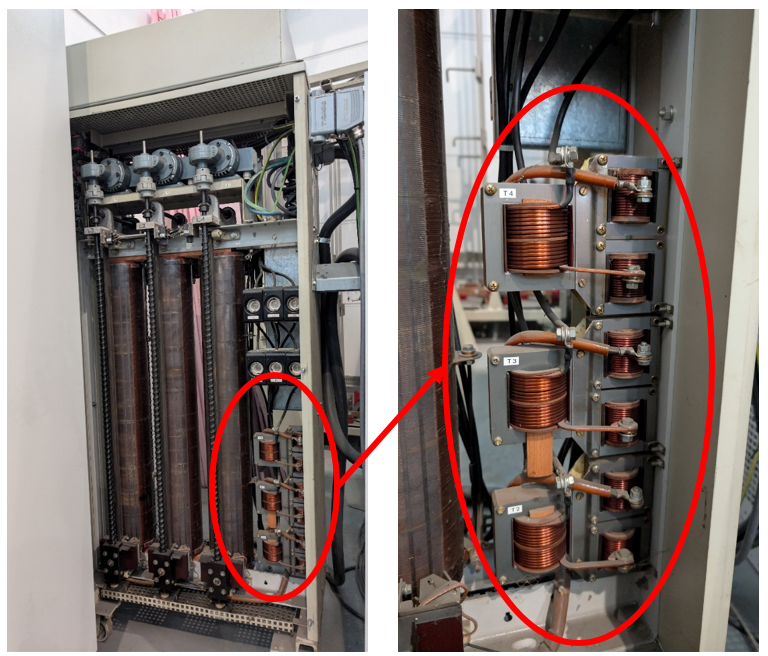
\includegraphics[width=0.92\textwidth]
    {03_Ressourcen/pic/Säulentrafo_Drosseln.png}
    \caption{Anordnung der induktiven Ausgleichselemente am
    Säulenstelltransformator (eigene Darstellung und eigene Aufnahmen)}
    \label{fig:ist_ausgleichselemente}
\end{figure}

Der Festtransformator setzt die einstellbare Spannung auf das
Niederspannungsniveau des Prüfstromkreises um. Nach Typenschild sind zwei
primärseitige Wicklungssysteme mit jeweils \SI{380}{\volt},
\SI{40}{\ampere} und \SI{15}{\kilo\volt\ampere} vorhanden. Für die
Sekundärseite sind \SI{6}{\volt} und \SI{5000}{\ampere} angegeben. Die
Typenschildangabe beschreibt den Bemessungspunkt des Transformators. Im
Prüfbetrieb wird die wirksame Ausgangsspannung durch den vorgeschalteten
Säulenstelltransformator verändert. Nach betrieblicher Bestandsaufnahme
steht dafür ein Bereich von näherungsweise \SIrange{0}{8}{\volt} zur
Verfügung
\parencite[Bestandsaufnahme: Festtransformator und
Betriebsbereich]{rj_pruefstand_2026}.

Bei Spannungsangaben im sekundärseitigen Prüfstromkreis ist zwischen der
Außenleiterspannung und der Spannung eines Außenleiters gegen den Sternpunkt
der Lastwiderstände zu unterscheiden. Der Sternpunkt ist ein interner
Rückführungspunkt des Prüfstromkreises und nicht mit einem Neutralleiter des
betrieblichen Netzes verbunden. In den nachfolgenden Untersuchungen wird die
jeweilige Bezugsart deshalb ausdrücklich angegeben.

Unmittelbar hinter dem Festtransformator ist für jeden Außenleiter ein
Stromwandler angeordnet. Die vorhandenen Stromwandler besitzen nach den
Anlagenangaben ein Übersetzungsverhältnis von

\begin{equation}
    \frac{I_\mathrm{p}}{I_\mathrm{s}}
    =
    \frac{\SI{5000}{\ampere}}{\SI{5}{\ampere}},
    \label{eq:ist_stromwandler_uebersetzung}
\end{equation}

eine Bemessungsleistung von \SI{10}{\volt\ampere} und die
Genauigkeitsklasse (0{,}2)
\parencite[Bestandsaufnahme: zentrale
Strommessung]{rj_pruefstand_2026}. Ihre Messwerte werden von der SPS für die
Ansteuerung der drei Motoren des Säulenstelltransformators verwendet. Der
Säulenstelltransformator ist damit das Stellglied einer übergeordneten
Stromregelung: Verändert wird die Spannung, zurückgeführt werden die hinter
dem Festtransformator gemessenen Außenleiterströme.

Das Anbindefeld bildet eine passive Hochstromschnittstelle zwischen der
Hochstromeinspeisung und unterschiedlichen Prüfkombinationen. Die in dieser
Arbeit betrachtete Prüfkombination besteht aus einem Leistungsschalterfeld
und einem MCC-Feld. Der eingespeiste Strom wird über den Leistungsschalter
auf die Hauptsammelschienen geführt. Von dort gelangt ein Anteil über die
vertikalen Verteilschienen zu den Abgangseinheiten des MCC-Feldes. Der
verbleibende Anteil fließt über die Hauptsammelschienen und eine
Kurzschlussbrücke zurück. Die Kurzschlussbrücke ermöglicht damit eine höhere
Belastung des Leistungsschalterfeldes und der Hauptsammelschienen, als sie
allein durch die Summe der MCC-Abgangsströme entstehen würde.

Für einen Außenleiter gilt im stationären sinusförmigen Betrieb die
Knotenregel in Zeigerdarstellung:

\begin{equation}
    \underline{I}_\mathrm{ges}
    =
    \underline{I}_\mathrm{KB}
    +
    \sum_{k=1}^{12}\underline{I}_{\mathrm{MCC},k}.
    \label{eq:ist_strombilanz}
\end{equation}

Dabei bezeichnet \(\underline{I}_\mathrm{KB}\) den Stromzeiger des
Kurzschlussbrückenpfads und \(\underline{I}_{\mathrm{MCC},k}\) den
Stromzeiger des jeweiligen MCC-Abgangs. Die häufig verwendete skalare
Addition der Effektivwerte ist nur dann eine hinreichende Näherung, wenn die
Phasenverschiebungen der parallelen Teilströme gegeneinander vernachlässigt
werden können.

Im bisherigen Prüfstand wurden für die kleinen Modulbaugrößen Prüfströme von
\SI{32}{\ampere} und \SI{63}{\ampere} eingesetzt. Die Abgänge der größeren
Modulbauformen wurden mit \SI{250}{\ampere}, \SI{400}{\ampere} und
\SI{630}{\ampere} belastet. Für die aus sechs A-Modulen, drei B-Modulen und
jeweils einem der drei größeren Abgänge bestehende Anordnung ergibt sich der
in Tabelle~\ref{tab:ist_belastungskonfiguration} aufgeführte Summenstrom.

\begin{table}[H]
    \centering
    \caption{Im bestehenden Prüfaufbau zugrunde gelegte und bereits
    erprobte Abgangsströme je Außenleiter}
    \label{tab:ist_belastungskonfiguration}
    \begin{tabular}{lccc}
        \toprule
        Abgangsgruppe & Anzahl & Prüfstrom je Abgang & Teilsumme \\
        \midrule
        A-Module & 6 & \SI{32}{\ampere} & \SI{192}{\ampere} \\
        B-Module & 3 & \SI{63}{\ampere} & \SI{189}{\ampere} \\
        \SI{250}{\ampere}-Abgang & 1 & \SI{250}{\ampere} &
        \SI{250}{\ampere} \\
        \SI{400}{\ampere}-Abgang & 1 & \SI{400}{\ampere} &
        \SI{400}{\ampere} \\
        \SI{630}{\ampere}-Abgang & 1 & \SI{630}{\ampere} &
        \SI{630}{\ampere} \\
        \midrule
        Gesamt & 12 & -- & \SI{1661}{\ampere} \\
        \bottomrule
    \end{tabular}
\end{table}

Das MCC-Feld ist in Geräte-, Sammelschienen- und Kabelanschlussräume
gegliedert. Die horizontalen Hauptsammelschienen führen den Gesamtstrom durch
das Feld, während die vertikalen Verteilschienen die parallel angeordneten
Abgangseinheiten versorgen. Nach der betrieblichen Projektdokumentation ist
das betrachtete Feld mit der inneren Unterteilung der Form 4a ausgeführt
\parencite[Bestandsaufnahme: konstruktive Ausführung des
MCC-Feldes]{rj_pruefstand_2026}. Die Sammelschienen sind damit von den
Funktionseinheiten und die Funktionseinheiten untereinander getrennt. Die
Anschlüsse äußerer Leiter befinden sich im selben Abteil wie die jeweils
zugeordnete Funktionseinheit
\parencite[Anhang~AA, Tab.~AA.1]{din_en_61439_2}.

Die lösbaren Abgangseinheiten werden über Adapter und federnde
Lyra-Kontakte mit den Verteilschienen verbunden. Innerhalb eines Abgangs
durchfließt der Strom die eingebauten Schalt-, Schutz- und
Stromerfassungsgeräte sowie die internen Verbindungen. Danach wird er über
die abgangsseitigen Kontakte und die Anschlussleitungen zu den außerhalb des
MCC-Feldes angeordneten Lastwiderständen geführt. Die Kontaktstellen,
Leitungen und Geräte tragen somit zur Ersatzimpedanz und zur Verlustleistung
des jeweiligen Strompfads bei. Ihre quantitative Ermittlung erfolgt in der
späteren Modellbildung; an dieser Stelle ist zunächst ihre Lage im realen
Strompfad maßgebend.

\begin{figure}[H]
    \centering
    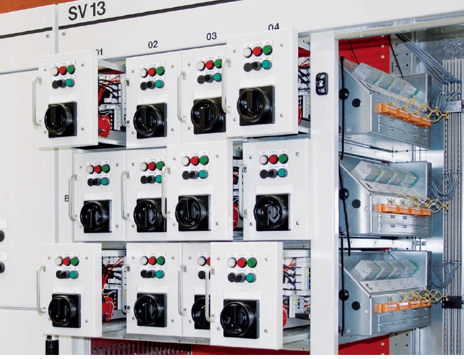
\includegraphics[width=0.95\textwidth]
    {03_Ressourcen/pic/MCC-Feld_Einschübe_Kabelanschlussraum.png}
    \caption{Geräteraum und Kabelanschlussraum des betrachteten
    MCC-Feldes mit den lösbaren Abgangseinheiten
    (betriebsinterne Darstellung)}
    \label{fig:ist_mcc_raeume}
\end{figure}

Die einstellbaren Lastwiderstände bestehen aus nichtrostenden
Stahlschienen. Je Phasenpfad sind zwei räumlich nebeneinander angeordnete
Schienen über eine verschiebbare Brücke elektrisch miteinander verbunden.
Der Strom fließt bis zur Position der Brücke über die erste Schiene und über
die zweite Schiene zum gemeinsamen Laststernpunkt zurück. Durch das
Verschieben der Brücke verändert sich die wirksame Leiterlänge und damit der
elektrische Widerstand des betreffenden Lastpfads. Die Brückenposition dient
im bestehenden Prüfaufbau als manuelle Stellgröße für den Abgangsstrom. Der
grundlegende Zusammenhang zwischen Leiterlänge und Widerstand wurde in
Abschnitt~\ref{sec:verlustleistung_temperaturkoeffizient} erläutert.

\begin{figure}[H]
    \centering
    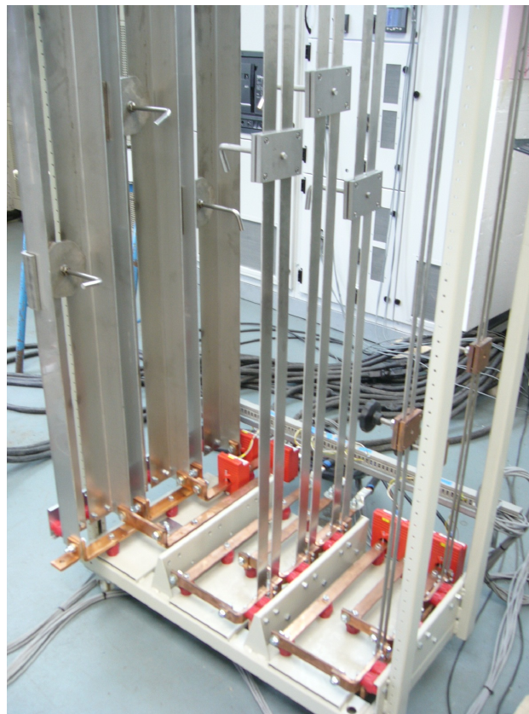
\includegraphics[height=0.65\textheight]
    {03_Ressourcen/pic/Widerstandswagen.png}
    \caption{Widerstandswagen mit verstellbaren Lastwiderständen aus
    nichtrostenden Stahlschienen (betriebsinterne Aufnahme)}
    \label{fig:ist_v2a_widerstandswagen}
\end{figure}

Der Ist-Zustand verbindet somit zwei unterschiedliche Arten der
Strombeeinflussung. Die übergeordneten Außenleiterströme werden durch die SPS
und den Säulenstelltransformator automatisch nachgeführt. Die Ströme der
einzelnen MCC-Abgänge werden zwar phasenbezogen gemessen, jedoch durch
manuelles Verstellen der jeweiligen Lastwiderstände eingestellt. Da die
Abgänge dieselbe Hochstromeinspeisung nutzen, wirken Änderungen der
gemeinsamen Speisespannung auf sämtliche parallelen Lastzweige.


% -----------------------------------------------------------------------------
% 3.2 Derzeitige Durchführung der Erwärmungsprüfung
% -----------------------------------------------------------------------------
\subsection{Derzeitige Durchführung der Erwärmungsprüfung}
\label{sec:durchfuehrung_ist}

Die betriebliche Durchführung lässt sich in die Vorbereitung der
Prüfanordnung, das Einstellen der Prüfströme, die mehrstündige
Erwärmungsphase und die abschließende Bewertung unterteilen. Vor Beginn der
Prüfung werden die vorgesehene Kombination aus Leistungsschalter- und
MCC-Feld aufgebaut, die Abgangseinheiten eingesetzt und die Lastleitungen
mit den zugeordneten Lastwiderständen verbunden. Der für die Belastung der
Hauptsammelschienen zusätzlich erforderliche Strompfad wird über die
Kurzschlussbrücke geschlossen. Anschließend werden die
Hochstromverbindungen, die Zuordnung der Messkanäle sowie die erforderlichen
Schutz- und Überwachungsfunktionen kontrolliert.

Zur Erfassung des Erwärmungsverlaufs werden Pt100-Widerstandsthermometer an
den für die Nachweisaufgabe festgelegten Messstellen angebracht. Dazu gehören
insbesondere stromführende Anschlüsse, Kontaktstellen, Schaltgeräte und
weitere thermisch relevante Komponenten der Prüfkombination. Die
Temperaturen werden gemeinsam mit den Strommesswerten in WinCC angezeigt und
zeitlich aufgezeichnet
\parencite[Bestandsaufnahme: Messwerterfassung und
Prüfablauf]{rj_pruefstand_2026}.

Die Strommessung erfolgt auf zwei Ebenen. Drei Stromwandler erfassen die
übergeordneten Außenleiterströme unmittelbar hinter dem Festtransformator.
Zusätzlich werden die drei Außenleiterströme jedes der zwölf MCC-Abgänge
gemessen. Damit stehen 36 phasenbezogene Modulstromwerte zur Überwachung der
Stromverteilung zur Verfügung. Diese 36 Messwerte sind von der Anzahl später
benötigter Stellglieder zu unterscheiden; die Zuordnung von Mess- und
Stellkanälen ist eine Fragestellung der Konzeptentwicklung.

Nach dem Einschalten wird der übergeordnete Prüfstrom mithilfe des
Säulenstelltransformators schrittweise auf den vorgesehenen Wert erhöht. Die
SPS verarbeitet die hinter dem Festtransformator gemessenen Ströme und
steuert die drei motorischen Antriebe an. Dadurch werden die dem
Festtransformator zugeführten Spannungen und in der Folge die
sekundärseitigen Außenleiterströme verändert.

Nachdem der übergeordnete Strom näherungsweise eingestellt ist, werden die
einzelnen Abgangsströme angepasst. Hierzu kontrolliert das Prüfpersonal die
in WinCC angezeigten Modulströme und verändert die Brückenpositionen der
zugeordneten Lastwiderstände. Eine Verkürzung der wirksamen Leiterlänge
verringert den Widerstand und erhöht den Abgangsstrom; eine Verlängerung
bewirkt das Gegenteil.

Die Einstellung erfolgt iterativ. Jede Änderung eines Lastwiderstands
verändert zunächst den Strom des zugehörigen Abgangs, zugleich aber auch die
Belastung der gemeinsamen Hochstromeinspeisung. Reagiert die übergeordnete
Stromregelung mit einer Spannungsänderung, werden ebenfalls die Ströme der
übrigen Abgänge beeinflusst. Nach einer Verstellung müssen deshalb nicht nur
der unmittelbar betroffene Abgang, sondern die gesamte Stromverteilung und
gegebenenfalls auch die Einstellungen weiterer Lastwiderstände erneut
kontrolliert werden.

Die mechanische Verstellung kann im derzeitigen Prüfablauf während der
Bestromung vorgenommen werden. Das niedrige Spannungsniveau des
Prüfstromkreises verringert zwar die Anforderungen an die elektrische
Isolation, darf jedoch wegen der hohen Ströme nicht mit einer allgemein
geringen Gefährdung gleichgesetzt werden. Thermische Belastungen,
Kontaktunterbrechungen, mögliche Lichtbogenbildung und elektrodynamische
Kräfte bleiben bei Eingriffen in den bestromten Lastkreis zu
berücksichtigen.

Mit der anfänglichen Einstellung beginnt die eigentliche Erwärmungsphase.
Während der mehrstündigen Belastung werden die Temperaturen, die
übergeordneten Außenleiterströme und die Modulströme fortlaufend erfasst. Die
zentrale Stromregelung führt weiterhin die hinter dem Festtransformator
gemessenen Ströme nach. Für die einzelnen Modulströme besteht dagegen keine
automatische Korrektur. Verändern sich die Lastzweigwiderstände infolge der
Erwärmung, müssen daraus resultierende Stromabweichungen vom Prüfpersonal
erkannt und durch erneutes Verschieben der Widerstandsbrücken ausgeglichen
werden.

Die nach Abschnitt~\ref{sec:erwaermungspruefung_norm} einzuhaltenden
Stromtoleranzen gelten bis zur maßgebenden Messwertaufnahme. Eine lediglich
zu Beginn erreichte Stromeinstellung reicht daher nicht aus. Die Prüfung wird
fortgeführt, bis der thermische Beharrungszustand erreicht ist. Dieser liegt
vor, wenn die Änderung der Temperaturerhöhung an den maßgebenden Messstellen
höchstens \SI{1}{\kelvin\per\hour} beträgt
\parencite[Abschn.~10.10.2.3.1]{din_en_61439_1}. Anschließend werden die
Temperatur- und Stromwerte dokumentiert, anhand der vorgegebenen Kriterien
bewertet und der Prüfstrom kontrolliert zurückgenommen.

Der derzeitige Ablauf kombiniert folglich eine automatische Nachführung der
übergeordneten Ströme mit einer manuellen Einstellung und Überwachung der
einzelnen Modulströme. Die wiederholte Kontrolle aller Abgänge bindet über
einen langen Zeitraum Personal und erschwert eine reproduzierbare
Einstellung der Stromverteilung.


% -----------------------------------------------------------------------------
% 3.3 Analyse der bestehenden Problematik
% -----------------------------------------------------------------------------
\subsection{Analyse der bestehenden Problematik}
\label{sec:analyse_problematik}

Die wesentliche Schwachstelle des bestehenden Prüfstands liegt nicht in der
grundsätzlichen Bereitstellung des Hochstroms, sondern in dessen Verteilung
auf die einzelnen MCC-Abgänge. Die vorhandene Regelung erfasst ausschließlich
die übergeordneten Außenleiterströme. Unterschiedliche Verteilungen der
Teilströme können jedoch zum selben Gesamtstrom führen. Die Einhaltung des
Sollwerts von \(I_\mathrm{ges}\) gewährleistet daher nicht, dass gleichzeitig
alle Abgangsströme ihren jeweiligen Sollwerten entsprechen.

Die nachfolgende Betrachtung erfolgt stellvertretend für einen Außenleiter.
Der Index \(k\) bezeichnet den jeweiligen MCC-Abgang. Dessen elektrische
Ersatzimpedanz lässt sich in einen Anteil der Abgangseinheit einschließlich
Kontakten und Leitungen sowie den temperaturabhängigen Lastwiderstand
zerlegen:

\begin{equation}
    \underline{Z}_{\mathrm{ges},k}(\vartheta_k)
    =
    \underline{Z}_{\mathrm{MCC},k}
    +
    \underline{Z}_{\mathrm{Ltg},k}
    +
    R_{\mathrm{V2A},k}(\vartheta_k).
    \label{eq:ist_gesamtimpedanz_abgang}
\end{equation}

Für den Strom des Abgangs gilt damit

\begin{equation}
    \underline{I}_{\mathrm{MCC},k}(\vartheta_k)
    =
    \frac{\underline{U}_\mathrm{B}}
    {\underline{Z}_{\mathrm{ges},k}(\vartheta_k)},
    \label{eq:ist_modulstrom_temperatur}
\end{equation}

wobei \(\underline{U}_\mathrm{B}\) die Spannung am gemeinsamen
Verteilungspunkt bezeichnet. Die Verwendung einer Impedanz ist erforderlich,
solange ein Blindanteil nicht nachweislich vernachlässigt werden kann. Die
spätere Ermittlung und begründete Vereinfachung der
MCC-Ersatzimpedanz erfolgt in der Modellbildung.

Die im Lastwiderstand umgesetzte Wirkleistung führt zu dessen Erwärmung. Für
den überwiegend ohmschen Widerstand gilt

\begin{equation}
    P_{\mathrm{V2A},k}
    =
    I_{\mathrm{MCC},k}^{2}R_{\mathrm{V2A},k}.
    \label{eq:ist_verlustleistung_v2a}
\end{equation}

Der verwendete nichtrostende Stahl besitzt im betrachteten Bereich einen
positiven Temperaturkoeffizienten. Unter Verwendung der in
Abschnitt~\ref{sec:verlustleistung_temperaturkoeffizient} eingeführten
linearen Näherung ergibt sich

\begin{equation}
    R_{\mathrm{V2A},k}(\vartheta_k)
    =
    R_{\mathrm{V2A},20,k}
    \left[
        1+
        \alpha_{20}
        \left(\vartheta_k-\SI{20}{\degreeCelsius}\right)
    \right].
    \label{eq:ist_v2a_temperaturabhaengigkeit}
\end{equation}

Wird die Spannung am Verteilungspunkt für die grundlegende Betrachtung als
konstant angenommen, folgt aus der Erwärmung die Ursache-Wirkungs-Kette

\begin{equation}
    \vartheta_k \uparrow
    \quad\Longrightarrow\quad
    R_{\mathrm{V2A},k} \uparrow
    \quad\Longrightarrow\quad
    I_{\mathrm{MCC},k} \downarrow.
    \label{eq:ist_kausalkette_stromdrift}
\end{equation}

Dieser Vorgang wird im weiteren Verlauf als thermisch bedingter Stromdrift
bezeichnet. Die Annahme einer konstanten Spannung dient ausschließlich der
Darstellung des lokalen Wirkzusammenhangs. Im realen Prüfstand verändert die
übergeordnete Stromregelung bei einer Änderung des Gesamtstroms die
gemeinsame Speisespannung. Diese Korrektur wirkt jedoch gleichzeitig auf den
Kurzschlussbrückenpfad und alle zwölf MCC-Abgänge. Sie kann deshalb keine
selektive Abweichung eines einzelnen Abgangs ausgleichen.

Der thermische Stromdrift fällt zwischen den Abgängen unterschiedlich aus.
Ursachen sind die verschiedenen Prüfströme, Leiterquerschnitte und wirksamen
Leiterlängen sowie Unterschiede der Kontakt-, Leitungs- und
Modulimpedanzen. Hinzu kommen unterschiedliche thermische Randbedingungen,
beispielsweise die Oberfläche, die Anordnung der Widerstände und die
Wärmeabgabe an die Umgebung. Eine einzige zentrale Stellgröße kann diese
individuellen Verläufe nicht gleichzeitig kompensieren.

Die manuelle Korrektur eines Abgangs führt zu einer weiteren Kopplung. Wird
die wirksame Länge seines Lastwiderstands verkürzt, steigt der betreffende
Abgangsstrom. Dadurch erhöht sich zunächst auch der übergeordnete Strom. Die
zentrale Regelung kann darauf mit einer Verringerung der gemeinsamen Spannung
reagieren, wodurch die Ströme der übrigen Abgänge sinken. Eine lokale
Korrektur kann somit neue Abweichungen in bereits eingestellten Zweigen
erzeugen. Dieser Zusammenhang erklärt den iterativen Charakter der
Stromeinstellung.

Eine Stromabweichung verändert außerdem die im Prüfling entstehende
Verlustleistung. Wird der elektrische Widerstand des betrachteten
Prüfpfads für einen Zeitpunkt als konstant angenommen, gilt

\begin{equation}
    \frac{P_k(I_k+\Delta I_k)}{P_k(I_k)}
    =
    \left(1+\frac{\Delta I_k}{I_k}\right)^2.
    \label{eq:ist_leistungsabweichung_stromabweichung}
\end{equation}

Bei einer Unterschreitung des Sollstroms um \SI{5}{\percent} verbleiben
damit nur

\begin{equation}
    \frac{P_k}{P_{k,0}}
    =
    (0{,}95)^2
    =
    0{,}9025
    \label{eq:ist_leistungsabweichung_beispiel}
\end{equation}

der vorgesehenen momentanen Verlustleistung. Die Verringerung beträgt somit
\SI{9.75}{\percent}. Bereits eine vergleichsweise kleine Stromabweichung kann
folglich den Erwärmungsverlauf und die erreichte Beharrungstemperatur
merklich beeinflussen. Die Stromnachführung ist daher nicht nur eine Frage
des Bedienkomforts, sondern eine Voraussetzung für vergleichbare und
reproduzierbare Prüfbedingungen.

Aus regelungstechnischer Sicht ist der Prüfstand als gekoppeltes
Mehrgrößensystem einzuordnen. Die gemeinsame Speisespannung wirkt als
zentrale Stellgröße auf sämtliche Lastpfade. Die einzelnen
Widerstandsbrücken stellen dezentrale Stellmöglichkeiten dar, werden jedoch
manuell betätigt. Der vorhandenen Regelung steht nur die Summe der
Teilströme als Regelgröße zur Verfügung; aus ihr kann die Verteilung auf die
einzelnen Abgänge nicht eindeutig rekonstruiert werden.

Damit ergeben sich vier wesentliche Defizite des Ist-Zustands:

\begin{itemize}
    \item Die einzelnen Abgangsströme werden nicht automatisch nachgeführt.
    \item Die Erwärmung der Lastwiderstände verursacht zeitlich
    unterschiedliche Stromabweichungen.
    \item Manuelle und zentrale Stellvorgänge beeinflussen über die
    gemeinsame Einspeisung auch andere Lastzweige.
    \item Die wiederholte Verstellung im bestromten Hochstromkreis verursacht
    Bedienaufwand und stellt erhöhte Anforderungen an einen sicheren
    Arbeitsablauf.
\end{itemize}

Eine Optimierung allein der vorhandenen Gesamtstromregelung kann diese
Defizite nicht beseitigen. Erforderlich ist eine gezielte Beeinflussung der
Stromverteilung auf die einzelnen MCC-Abgänge.


% -----------------------------------------------------------------------------
% 3.4 Anforderungen an das Optimierungskonzept
% -----------------------------------------------------------------------------
\subsection{Anforderungen an das Optimierungskonzept}
\label{sec:anforderungen_optimierung}

Aus der Analyse werden im Folgenden die Anforderungen an die zu
untersuchenden Stellkonzepte abgeleitet. Die Anforderungen werden zunächst
vom später gewählten Wirkprinzip getrennt. Dadurch können ein zusätzlicher
verstellbarer Widerstand, ein induktiver Stellpfad und
transformatorgestützte Lösungen in Kapitel~\ref{chap:entwicklung_stellkonzept}
an denselben Kriterien beurteilt werden.

Die zentrale funktionale Anforderung ist die automatische Nachführung der
einzelnen Abgangsströme. Für jeden Außenleiter jedes MCC-Abgangs muss der
Iststrom erfasst und mit dem vorgesehenen Sollwert verglichen werden. Bei
zwölf dreiphasigen Abgängen ergeben sich

\begin{equation}
    n_\mathrm{I}
    =
    12\cdot 3
    =
    36
    \label{eq:anzahl_modulstromkanaele}
\end{equation}

phasenbezogene Strommesswerte. Die Zahl der Messkanäle legt die Zahl der
mechanisch oder elektrisch unabhängigen Stellglieder noch nicht fest. Eine
gemeinsame dreiphasige Stellbewegung ist nur dann geeignet, wenn die
Abweichungen aller drei Außenleiter innerhalb der zulässigen Grenzen bleiben.
Andernfalls ist eine phasenselektive Stellwirkung erforderlich.

Für die künftige Belastungskonfiguration sollen die sechs A-Module mit
jeweils \SI{40}{\ampere} und die drei B-Module mit jeweils
\SI{70}{\ampere} betrieben werden. Die Prüfströme der drei größeren Abgänge
bleiben bei \SI{250}{\ampere}, \SI{400}{\ampere} und
\SI{630}{\ampere}. Damit steigt der vorgesehene Summenstrom der zwölf
MCC-Abgänge gegenüber der bisher erprobten Konfiguration von
\SI{1661}{\ampere} auf \SI{1730}{\ampere} je Außenleiter.

\begin{table}[H]
    \centering
    \caption{Für die Optimierung vorgesehene Belastungskonfiguration je
    Außenleiter}
    \label{tab:mcc_belastungskonfiguration}
    \begin{tabular}{lccc}
        \toprule
        Abgangsgruppe & Anzahl & Sollstrom je Abgang & Teilsumme \\
        \midrule
        A-Module & 6 & \SI{40}{\ampere} & \SI{240}{\ampere} \\
        B-Module & 3 & \SI{70}{\ampere} & \SI{210}{\ampere} \\
        \SI{250}{\ampere}-Abgang & 1 & \SI{250}{\ampere} &
        \SI{250}{\ampere} \\
        \SI{400}{\ampere}-Abgang & 1 & \SI{400}{\ampere} &
        \SI{400}{\ampere} \\
        \SI{630}{\ampere}-Abgang & 1 & \SI{630}{\ampere} &
        \SI{630}{\ampere} \\
        \midrule
        Gesamt & 12 & -- & \SI{1730}{\ampere} \\
        \bottomrule
    \end{tabular}
\end{table}

Der zugehörige Summenstrom beträgt

\begin{equation}
\begin{aligned}
    I_{\mathrm{MCC},\Sigma}
    &=
    6\cdot\SI{40}{\ampere}
    +3\cdot\SI{70}{\ampere}
    +\SI{250}{\ampere}
    +\SI{400}{\ampere}
    +\SI{630}{\ampere}
    \\
    &=
    \SI{1730}{\ampere}.
\end{aligned}
\label{eq:mcc_summenstrom_belastungskonfiguration}
\end{equation}

\begin{figure}[H]
    \centering
    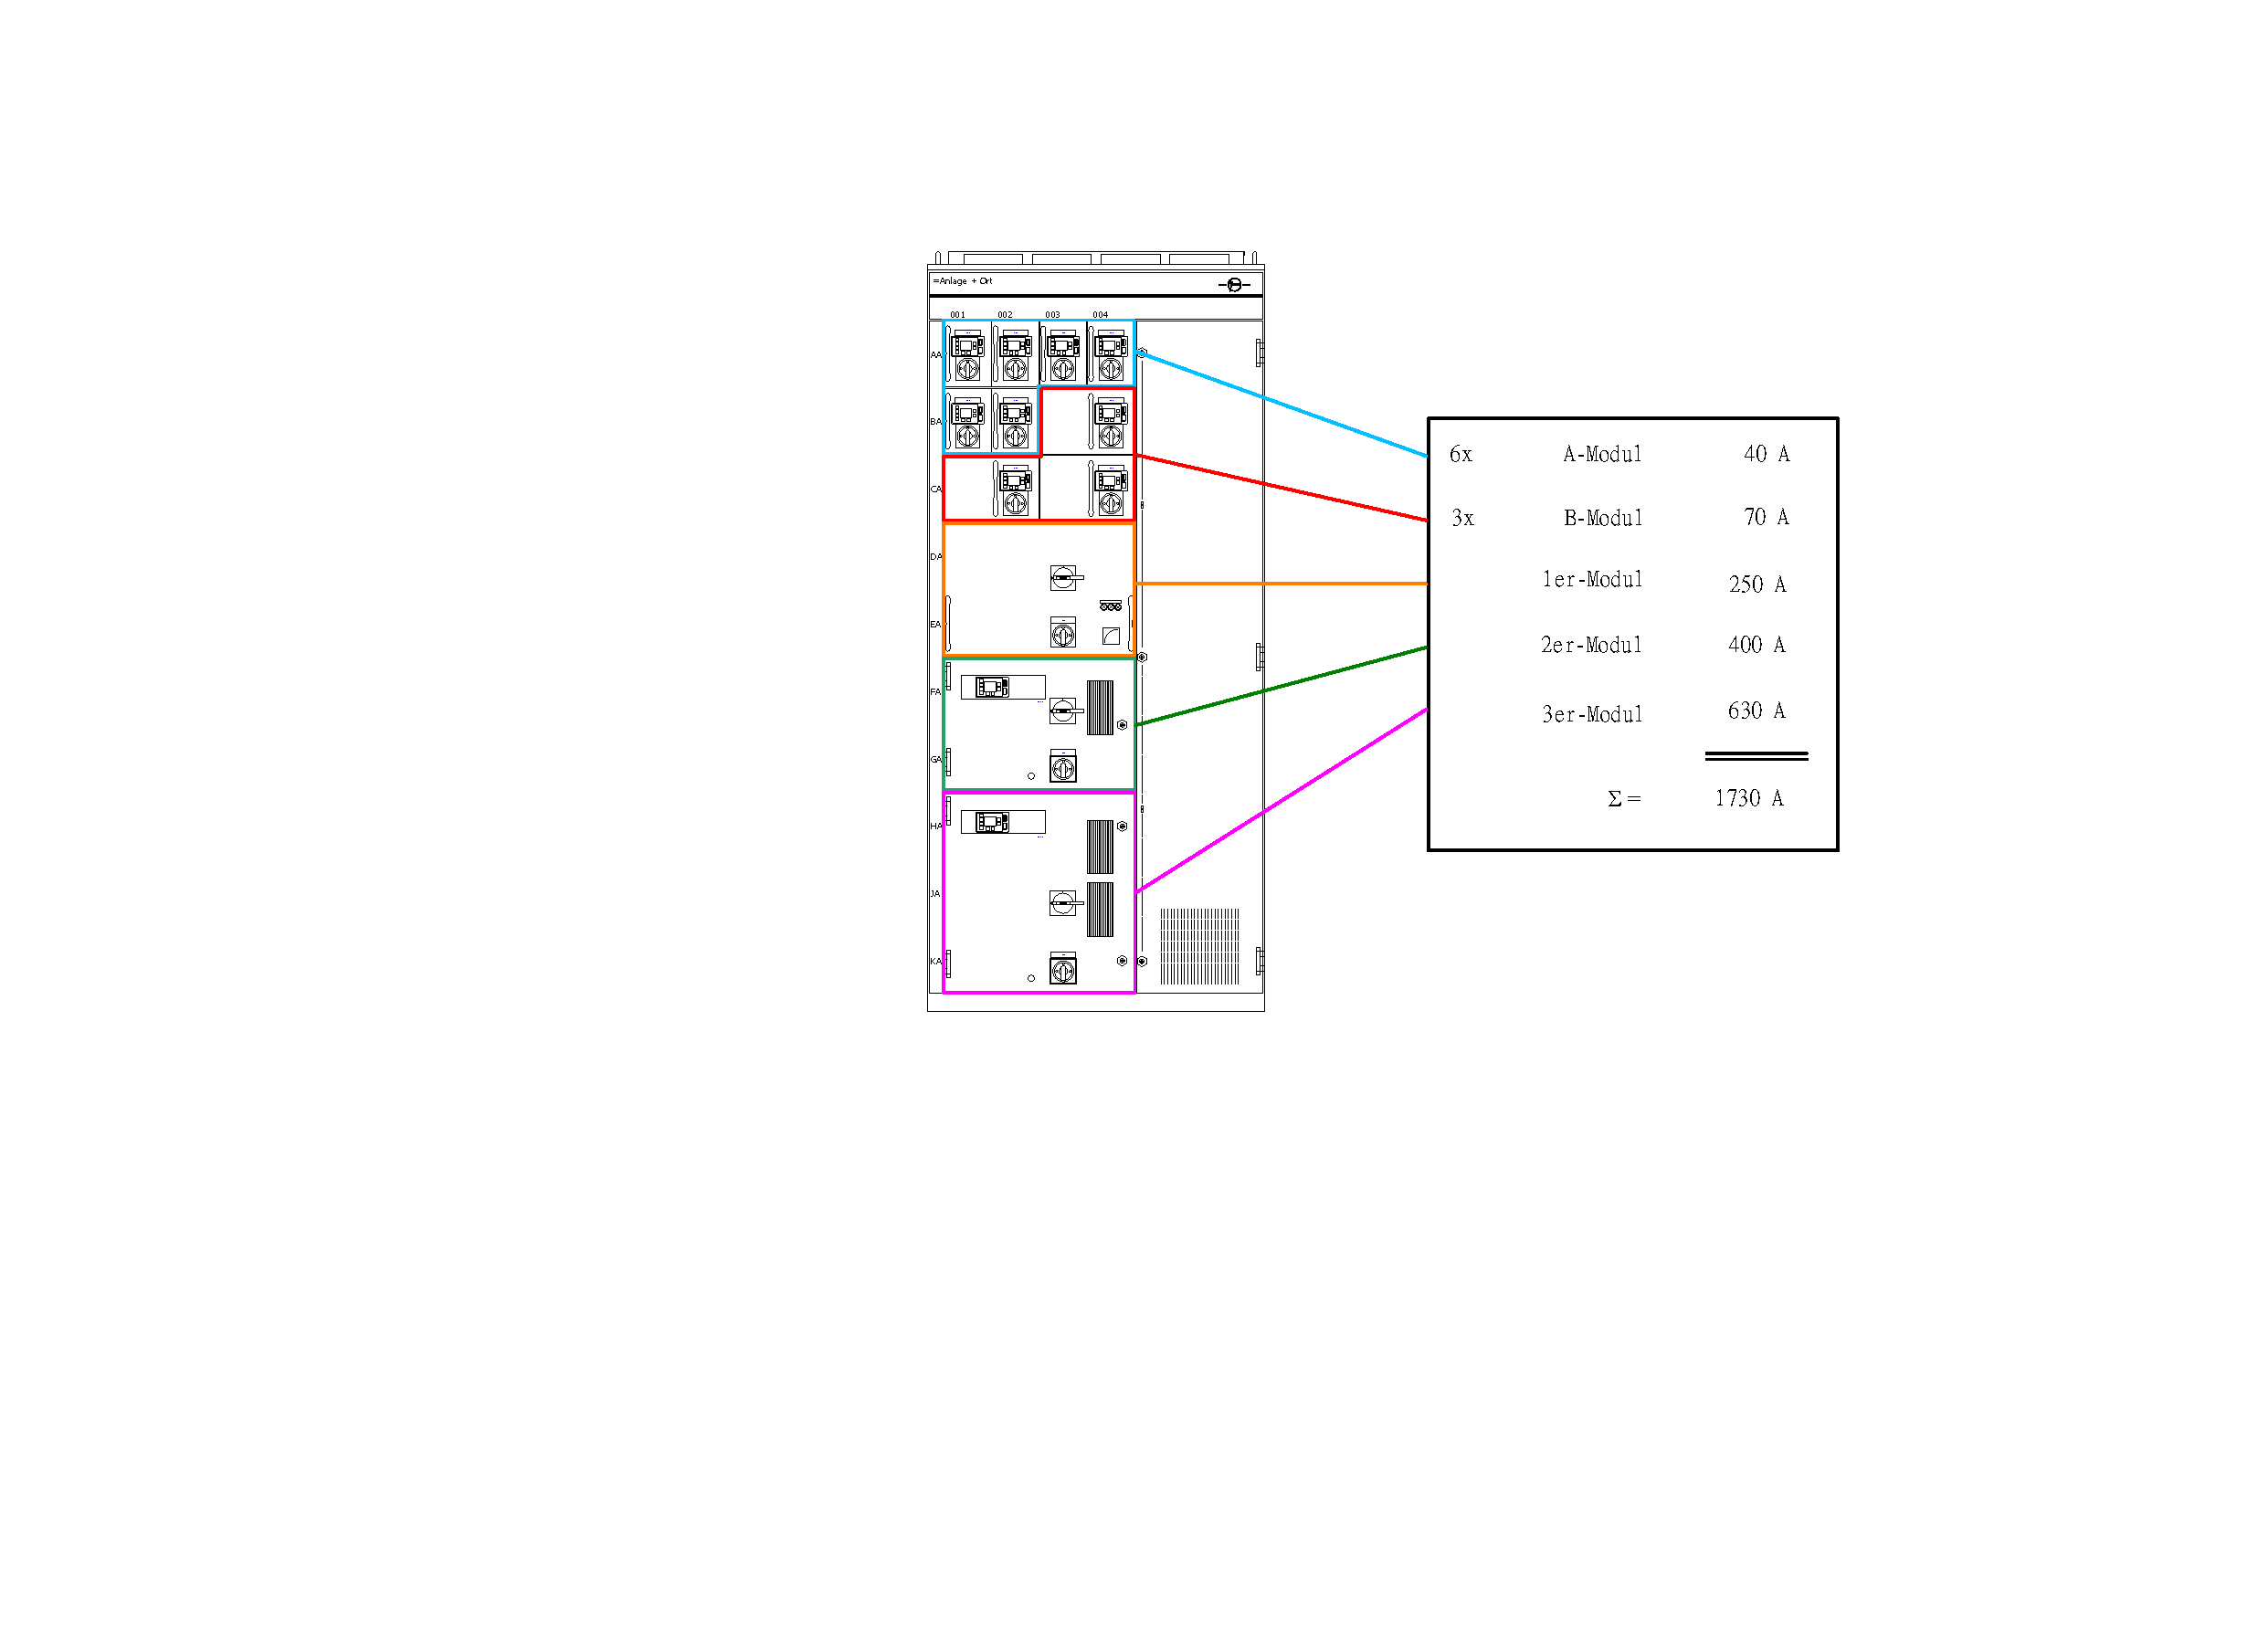
\includegraphics[width=\textwidth]
    {03_Ressourcen/pic/Frontansicht_MCC_Xournal.pdf}
    \caption{Für die Optimierung vorgesehene Modulbestückung des
    MCC-Feldes}
    \label{fig:mcc_modulbestueckung}
\end{figure}

Neben dem Sollstrombereich ist eine ausreichende Stellreserve erforderlich.
Das Stellglied muss zunächst die Einstellung des Sollstroms ermöglichen und
anschließend die temperaturbedingte Änderung der Lastzweigimpedanz
ausgleichen können. Es darf weder im kalten Ausgangszustand noch bei der
größten zu erwartenden Betriebstemperatur an einer mechanischen,
elektrischen oder regelungstechnischen Grenze betrieben werden. Der
quantitativ erforderliche Stellbereich wird auf Grundlage der Modellbildung
und der Simulation bestimmt.

Die vorhandene Hochstromeinspeisung und ihre übergeordnete Regelung sind bei
der Entwicklung zu berücksichtigen. Eine dezentrale Stellbewegung darf keine
unzulässigen Stromabweichungen in anderen Abgängen hervorrufen. Gleichzeitig
müssen die Dynamiken der zentralen und der dezentralen Stellvorgänge so
aufeinander abgestimmt werden, dass keine bleibenden Schwingungen oder
fortlaufenden gegenläufigen Stellbewegungen entstehen. Welche Regelgröße dem
Säulenstelltransformator im optimierten Aufbau zugeordnet wird, ist dabei
nicht vorwegzunehmen, sondern für das jeweilige Konzept zu untersuchen.

Die zusätzlichen Komponenten müssen in den vorhandenen Prüfstand integrierbar
und für den mehrstündigen Dauerbetrieb geeignet sein. Ihre Verlustleistung
und Eigenerwärmung dürfen das thermische Verhalten des Prüflings nicht
unzulässig beeinflussen. Wärme erzeugende Betriebsmittel sind deshalb nach
Möglichkeit außerhalb der für den Erwärmungsnachweis maßgebenden thermischen
Systemgrenze anzuordnen. Leiter, Wicklungen, Kontaktstellen und Stellglieder
sind für die jeweiligen Dauerströme und die auftretenden Temperaturen zu
dimensionieren.

Die automatische Nachführung soll Eingriffe in den bestromten Lastkreis
vermeiden. Elektrische und mechanische Stellgrenzen müssen überwacht werden.
Bei einem fehlerhaften oder fehlenden Messsignal darf die Regelung keine
unkontrollierte Erhöhung des Abgangsstroms verursachen. Abhängig vom
Wirkprinzip ist die Stellbewegung zu sperren, ein nachgewiesener sicherer
Zustand einzunehmen oder der betroffene Kanal kontrolliert abzuschalten.

Für die betriebliche Nutzung sollen die vorhandene SPS- und WinCC-Umgebung
soweit technisch zweckmäßig weiterverwendet werden. Mindestens Sollstrom,
Iststrom, Regeldifferenz, Stellgröße und Grenzzustände müssen je Regelkanal
erfasst und zeitlich aufgezeichnet werden können. Eine definierte
Stellposition muss reproduzierbar anfahrbar sein, damit sich Prüfabläufe
wiederholen und Ergebnisse nachvollziehbar dokumentieren lassen.

Tabelle~\ref{tab:anforderungen_optimierung} fasst die aus der Analyse
abgeleiteten Bewertungskriterien zusammen. Die quantitative Konkretisierung
erfolgt dort, wo Mess- oder Modelldaten erforderlich sind, in den
nachfolgenden Kapiteln.

\begin{table}[H]
    \centering
    \caption{Anforderungen und Bewertungskriterien für die
    Konzeptentwicklung}
    \label{tab:anforderungen_optimierung}
    \small
    \begin{tabular}{p{0.06\textwidth}p{0.27\textwidth}p{0.55\textwidth}}
        \toprule
        ID & Anforderung & Bewertungskriterium \\
        \midrule
        A1 & Sollwerttreue &
        Einhaltung der in Abschnitt~\ref{sec:erwaermungspruefung_norm}
        festgelegten Stromtoleranzen bis zur Messwertaufnahme \\
        A2 & Strombereich &
        Nachführung der vorgesehenen Abgangsströme von
        \SIrange{40}{630}{\ampere} \\
        A3 & Phasenbezogene Erfassung &
        Verarbeitung aller 36 Modulstrommesswerte und Erkennung
        verbleibender Phasenabweichungen \\
        A4 & Stellbereich und Reserve &
        Sollstrom im kalten Zustand und thermische Nachführung ohne
        Anschlagbetrieb \\
        A5 & Beherrschung der Kopplung &
        Keine unzulässige Beeinflussung anderer Abgänge und stabiles
        Zusammenwirken mit der übergeordneten Regelung \\
        A6 & Dauerbetriebsfähigkeit &
        Zulässige elektrische und thermische Beanspruchung während der
        gesamten Prüfdauer \\
        A7 & Rückwirkungsarme Integration &
        Keine unzulässige zusätzliche Erwärmung oder Veränderung der
        Randbedingungen des Prüflings \\
        A8 & Automatisierbarkeit &
        Elektrische Ansteuerung, erfassbare Stellposition und Einbindung in
        SPS und WinCC \\
        A9 & Betriebssicherheit &
        Grenzüberwachung und definierter Zustand bei Mess- oder
        Stellfehlern \\
        A10 & Reproduzierbarkeit und Bedienaufwand &
        Wiederholbare Stellzustände und weniger manuelle Eingriffe während
        der Erwärmungsphase \\
        \bottomrule
    \end{tabular}
\end{table}

Die Anforderungen legen noch kein bestimmtes Stellprinzip fest. In
Kapitel~\ref{chap:entwicklung_stellkonzept} werden deshalb zunächst vier
technische Ansätze untersucht: ein zusätzlicher motorisch verstellbarer
Widerstandspfad, ein induktiver Parallelzweig mit veränderlichem
magnetischem Kreis sowie zwei Varianten mit einem zusätzlichen Transformator
und motorisch verstellbaren Widerständen. Erst der anschließende Vergleich
entscheidet, welche Konzepte in der Modellbildung und Simulation weiter
verfolgt werden.
